В данной работе для изучения микролинзирования используется вычислительная программа {\tt{microlens}} (\cite{wambsganss1999}), которая моделирует методом обратной трассировки лучей (\textit{inverse ray tracing}) распределение каустик в плоскости источника, основываясь на распределении звёзд в плоскости линзы. Выходными данными этой программы являются карты микрокаустик, содержащие значения обусловленного микролинзированием усиления. Основными параметрами для каждой карты являются поверхностные плотности звёзд $\kappa_*$ и непрерывно распределенной тёмной материи $\kappa_c$ в линизирующей галактике, внешний сдвиг $\gamma$, учитывающий вклад гравитационного потенциала скопления галактик, а также функция масс звёзд. 

\begin{figure}[H]
    \centering
	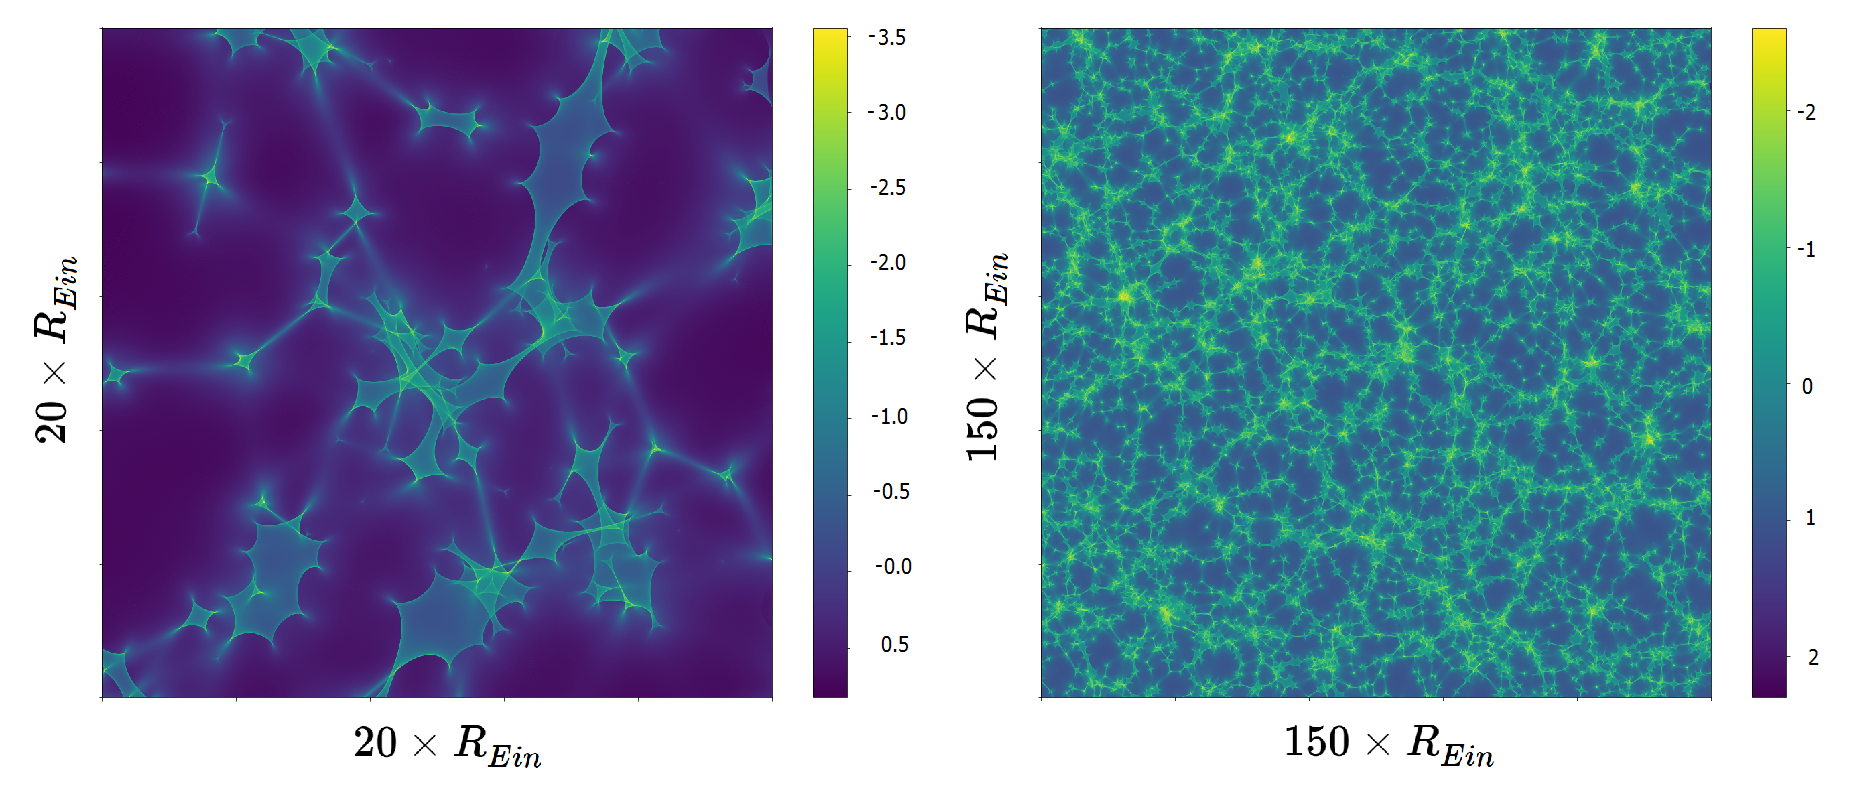
\includegraphics[scale=0.22]{pics/maps_example.png}
	\caption{Карты микрокаустик. Количество звёзд-линз слева - 313, справа - 14526. Цветовая шкала (в единицах звёздных величин) показывает, как увеличивается или ослабляется яркость источника вследствие микролинзирования только. \label{fig:micromaps}} 
\end{figure}
Здесь и далее для простоты предполагается, что все звезды в галактике имеют одинаковую массу, которая равна массе Солнца. На Рисунке \ref{fig:micromaps} приведены примеры результатов выполнения программы {\tt{microlens}} - карты усилений для двух различных значений количества звёзд, вызывающих микролинзирование. Светлые области означают, что источник усиливается, находясь в них, тёмные - что ослабляется. Видно, что а) сеть каустик намного богаче при большем количестве звёзд-линз, б) по всей карте усиление меняется и почти нигде не остаётся таким, каким его предсказывает модель линзы, то есть в отсутствие микролинзирования.